%%%design overview over libpninx

The aim of \pninx\ is to provide an easy to use but yet powerful interface
to write Nexus files from C++. Although the Nexus group already provides 
an binding of their Nexus API (NAPI) for C++, this is not much more than a 
thin wrapper around the Nexus C API. Thus the native C++ API does not espose
many of the features a C++ programmer would expect from an API. 
\pninx\ is an approach to overcome the limitations of the native C++ API 
and provide you with all the object oriented features that C++ exposes.

This chapter presents the general design of the API. Every user of the API is
highly encouraged to read this chapter as it contains the basic information 
required to use the API. In particular 
section~\ref{section:nxfield_design} should be read by all users of \pninx. 

\section{Nexus and HDF5}

There is some confusion about how Nexus and HDF5 are related to each other. 
The reason for this confusion is mostly due to the fact that Nexus is considered
by many people to be a physical file format of its own. Indeed, Nexus is only a
set of rules and conventions how data should be organized (we will see later
what this means). However, in the end data is writing using one of several
physical file formats supported by Nexus. These formats are XML, HDF4, and last
but not least HDF5. As Nexus describes the structure of data (not the way how it
will be stored on disk) the file format used to store data according to the
Nexus standard must provide some kind of structuring mechanisms as it is the
case for the formats mentioned above. 
While the native Nexus APIs support all these physical file formats \pninx\
only supports HDf5. However, as the other tow (HDF4 and XML) are available
mostly due to historical reasons, this is not a serious limitation. 

HDF5 is a binary file format which is primarily developed  to store large
amounts of numerical data. 
An HDF5 file can be considered pretty much like file system. The data is stored 
in objects called {\em datasets}. In simplest case a dataset is a
multi-dimensional array holding data of a particular type. The datasets can be 
organized in {\em groups}. Thus, to come back to the image of a file system 
the datasets represent files where the groups can be considered as directories.
For those who are more familiar with scientific software development a dataset
can also be imagined as a {\tt numpy} array in Python or as a numerical array 
in Fortran. Such arrays have a data-type and a shape. The later one holds the 
number of elements along each dimension of the array.
As the datasets are organized by groups each of them can be addressed by a Unix
like path (we are back again in the file-system picture). In the 

Attributes can be attached to groups and datasets in an HDF5 file. One  can
imagine attributes as kind of tags that can be stuck on an object. 
Attributes by them self can be strings, arrays or whatever other data you might 
can think of. 


\section{Classes and implementation}\label{section:classes_implementation}

%%%----------------------------------------------------------------------------
\begin{figure}[tb]
\centering
\begin{minipage}[t]{0.4\linewidth}
\centering
\resizebox{\linewidth}{!}{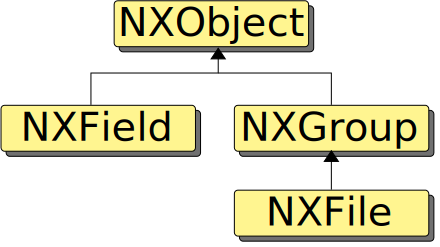
\includegraphics{pics/class_inheritance.pdf}}
\caption{{\small\label{fig:class_inheritance}
There are only four major objects: \nxobject, \nxfield, \nxgroup, and 
\nxfile. Which are all derived from \nxobject. 
}}
\end{minipage}
\hfill
\begin{minipage}[t]{0.59\linewidth}
\centering
\resizebox{\linewidth}{!}{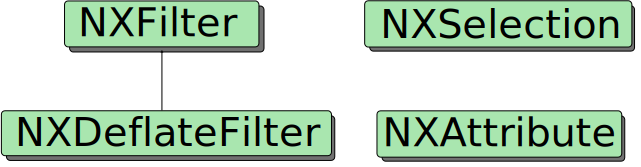
\includegraphics{pics/helper_classes.pdf}}
\caption{{\small\label{fig:helper_classes} 
Helper classes
}}
\end{minipage}
\end{figure}
%%%----------------------------------------------------------------------------
To keep the API simple, only a few classes are exposed. These classes and their 
relationship among each other are depicted in Fig.~\ref{fig:class_inheritance}. 
The top-level class is \nxobject. It provides the common functionality 
of every object within the API. \nxfield\ and \nxgroup\ divide the classes 
available in two groups: the former class is the base for all data holding
objects while the latter is the fundamental container class. 
\nxgroup\ corresponds with some extensions to a group in an HDF5 file or to 
a directory in a file-system (if you like this picture more). 

\begin{description}
\item[\nxgroup] the standard container to hold all kinds of objects
\item[\nxfield] the data holding objects
\item[\nxfile] object representing a data file.
\end{description}
\nxfile is a descendant of \nxgroup\ as can be seen in
Fig.~\ref{fig:class_inheritance}. Thus it posses all the functionality that 
\nxgroup\ has aside from those methods necessary for file handling. 
\pninx\ uses HDF5 to write data to disk. However, you do not have to know 
anything about HDF5. No low level HDF5 calls are necessary. Everything is 
masked by the three objects mentioned above. 
In order to do so a Bridge pattern~\cite{book:gof} was used for the
implementation. The idea was to separate the interface provided to the user from the 
concrete interface used to communicate with the HDF5 library. 
This allows us to change the HDF5 backend completely without changing 
user code using the library (maybe recompilation is needed - but this is not as
bad as changing code). This gives us much more freedom in maintaining \pninx.
The bridge pattern is not implemented as shown in \cite{book:gof} but rather 
by using a template approach as shown  in \cite{book:alexandrescu}.
Hence the code remains free of pointers which makes it much more readable. 
Furthermore it should be mentioned that the \pninx\ heavily relies on features 
provided by the C++11 standard. Thus, an actual compiler is required to 
build the library (for {\tt gcc} a version larger or equal $4.4$ is required).
 

\section{Supported datatypes}

\begin{table}[tb]
\centering
\begin{tabular}{l|c|l||l|c|l}
 name & size (Bit) & description & name & size (Bit) & description \\
 \hline
 {\tt UInt8} & $8$ & unsigned integer & {\tt Float32} & $32$ & floating point \\
 {\tt Int8}  & $8$ & signed integer &   {\tt Float64} & $64$ & floating point \\
 {\tt UInt16} & $16$ & unsigned integer & {\tt Float128} & $128$ & floating
 point\\
 {\tt Int16} & $16$ & signed integer & {\tt Complex32} & $64$ & complex floating
 point \\
 {\tt UInt32} & $32$ & unsigned integer & {\tt Complex64} & $128$ & complex
 floating point \\
 {\tt Int32} & $32$ & signed integer & {\tt Complex128} & $256$ & complex
 floating point \\
 {\tt UInt64} & $64$ & unsigned integer & & & \\
 {\tt Int64} & $64$ & signed integer & & & \\
\hline
\end{tabular}
\caption{{\small\label{tab:numeric_types} Numerical data-types supported by
\pninx. The complex floating point types are instances of the {\tt
std::complex<T>} template for the  {\tt Float32}, {\tt Float64}, and {\tt
Float128} types respectively.}}
\end{table}

\pninx\ supports a whole bunch of data-types. The numeric types are shown in 
Tab.~\ref{tab:numeric_types}. \pninx supports all types supported by the Nexus
standard too. In addition there is support for complex numbers and for $128$ Bit
floating point numbers. The complex numbers are instances of the 
{\tt std::complex<T>} template provided by C++.
In addition to the numerical types there is support for string and binary data. 
Strings are represented by the {\tt String} type which is basically nothing else
than a {\tt typedef} to {\tt std::string} included in the C++ standard library.
The binary type {\tt Binary} is slightly more complex. In the official Nexus
standard binary data is represented by {\tt unsigned char}. This has several 
disadvantages. The first is that binary data looks completely the same 
for the compiler as {\tt UInt8} (being itself a {\tt typedef} to {\tt unsigned
char}). This makes it impossible to distinguish this two types in template
parameters. In addition all arithmetic operators are defined for {\tt unsigned
char} which would make it possible to treat binary data as numbers which is
definitely what we want. To circumvent this problem a special template 
{\tt BinaryType<T>} was defined and the type {\tt Binary} is nothing else 
than a {\tt typedef} to {\tt BinaryType<unsigned char>}. The resulting type is
binary compatible with {\tt unsigned char} however, since no arithmetic
operators are exposed such operations are impossible with binary data. 
The compiler would not even compile code that tries to do such things. 


\section{The \nxfield\ class}
%%%============================================================================
\begin{figure}[tb]
\centering
\begin{minipage}[t]{0.25\linewidth}
\centering
\resizebox{\linewidth}{!}{\includegraphics{pics/array.pdf}}
\caption{{\small\label{fig:array}A two dimensional \nxfield\ before growing. }}
\end{minipage}
\hspace{0.01\linewidth}
\begin{minipage}[t]{0.3\linewidth}
\centering
\resizebox{\linewidth}{!}{\includegraphics{pics/array_grow.pdf}}
\caption{{\small\label{fig:array_grow}The \nxfield\ after growth along dimension
$0$ by $2$ elements.}}
\end{minipage}
\hspace{0.01\linewidth}
\begin{minipage}[t]{0.36\linewidth}
\centering
\resizebox{\linewidth}{!}{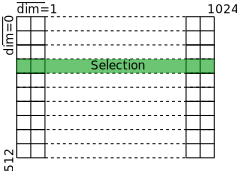
\includegraphics{pics/selection.pdf}}
\caption{{\small\label{fig:selection}\nxselection\ object allow to read only 
portions of an \nxfield. This is sometimes useful where one is not interested in
the entire data.}}
\end{minipage}
\end{figure}
%%%============================================================================

The class a user of \pninx\ most often has to deal with is \nxfield. 
Thus a short introduction to the concepts behind \nxfield\ should be given here.
A field is basically nothing else than a dataset in the HDF5 world. 
It represents a multi-dimensional array of data of a particular type stored on
disk. The data-type can be any of the types supported by \pninx\ and described
in the previous section. 
Figure~\ref{fig:array} shows a $2$-dimensional field. The number of dimensions
of a field is determined at creation time. However, the number of elements along
each dimension can be extended (not reduced, due to limitations of HDF5) during 
the entire lifetime of the \nxfield\ object. This process is called {\em
growth}. A \nxfield\ object can grow along a single dimension by certain number
of elements. An example of such an operation is shown in
Fig.~\ref{fig:array_grow} where the field from Fig.~\ref{fig:array} is expanded
by two elements along dimension $0$. 
It is important to note that the ordering of elements in a \nxfield\ object
follows the {\tt C}-convention. This means that the last index varies fastest.

A helper class which is of particular importance is the \nxselection\ class. 
It is mentioned here because it is very closely related to \nxfield\ objects.
Selections allow for partial IO. This means only a small portion of the data
stored in an \nxfield\ object is read or written. Figure~\ref{fig:selection}
shows the basic concept of a selection applied to a $2$-dimensional field. 
\nxselection\ objects as will be shown later are totally bound to the \nxfield\
object which created them. This is important in  as so far that a selection can
be applied only to the field that created it.
 

